\documentclass[11pt]{article}

% -----------------------------------
% Page Layout
% -----------------------------------
\usepackage[a4paper,margin=1in]{geometry}
\usepackage{needspace}
% -----------------------------------
% Fonts (Clean IEEE-like)
% -----------------------------------
\usepackage{newtxtext,newtxmath} % Times-like font
\usepackage{float}
% -----------------------------------
% Spacing
% -----------------------------------

\usepackage{tikz}
\usetikzlibrary{positioning,arrows.meta,shapes.geometric}
\usepackage{algorithm}
\usepackage{algpseudocode}

\setlength{\textfloatsep}{0pt}
\setlength{\abovecaptionskip}{0pt}
\setlength{\belowcaptionskip}{0pt}
\raggedbottom \setlength{\parskip}{0em}


\usepackage{titlesec}


\titlespacing*{\section}
  {0pt}{0em}{0em}


\usepackage{setspace}
\setstretch{1.2}  % adjust 1.2–1.4 as needed
\setlength{\parskip}{0.6em}
\setlength{\parindent}{0pt}


% \makeatletter
% \renewcommand{\section}{\@startsection
%   {section}{1}{0mm}
%   {-\baselineskip}
%   {0.5\baselineskip}
%   {\normalfont\large\bfseries}}
% \makeatother

\raggedbottom
\clubpenalty=1000
\widowpenalty=1000



% -----------------------------------
% Packages
% -----------------------------------
\usepackage{amsmath,amssymb}
\usepackage{graphicx}
\usepackage{booktabs}
\usepackage{enumitem}
\usepackage[numbers,sort&compress]{natbib}
\usepackage{hyperref}
\hypersetup{
    colorlinks=true,
    linkcolor=black,
    citecolor=black,
    urlcolor=black
}

% ---------- Title ----------
\title{Learning Topology-Aware Cooperative Caching Policies for IoT Edge Networks}
\author{
    Abdullah Al Mujahid, Asir Abrar, Monideepa Kundu Sinthi
}
\date{April 02, 2026}
\usepackage{titling}

% Tighten vertical spacing inside title block
\pretitle{\begin{center}\Large\bfseries}
\posttitle{\par\end{center}\vspace{-1.5em}}

\preauthor{\begin{center}\normalsize}
\postauthor{\par\end{center}\vspace{-2em}}

\predate{\begin{center}\normalsize}
\postdate{\par\end{center}\vspace{-2em}}

\setlength{\droptitle}{-0.8cm} % optional: pulls whole block upward



\begin{document}



\begingroup
\setstretch{0.90} % prevent your 1.5 spacing from inflating the title block
\maketitle
\endgroup

\begin{abstract}
This project studies cooperative content caching for IoT edge networks whose effective topology changes because users move among access points. We model edge nodes as a weighted mobility graph, synthesize content demand with Zipf popularity and spatial locality, and optimize cache placement under access latency, redundancy, replication, and relocation costs. The proposed pipeline combines a topology-aware greedy warm start with a compact Deep Q-Network (DQN) refinement stage. A reproducible implementation is provided with dataset access tooling, trace-compatible fallback generation, graph construction, perturbation sampling, baselines, metrics, and report-ready result assets. In the measured run included with this repository, the hybrid method achieves the lowest objective value across all perturbation settings and improves the nominal objective from 2.633 for topology-aware greedy to 2.414 while maintaining a 0.994 hit ratio.
\end{abstract}

\textbf{Keywords:} edge caching, IoT, cooperative caching, mobility graph, Zipf demand, deep reinforcement learning, DQN.


\needspace{4\baselineskip}
% \section{Introduction}

The expansion of the Internet of Things (IoT), together with the deployment of data-intensive applications over 5G and emerging 6G networks, has increased the demand for low-latency, high-throughput, and reliable data access at the network edge. Applications such as smart city monitoring, autonomous transportation, industrial automation, augmented reality, and large-scale sensor networks continuously generate and consume delay-sensitive, making centralized cloud processing inefficient due to latency, backhaul congestion, and scalability limitations.

Edge computing address this challenges by bringing computation and storage resources closer to end users. Among various edge computing mechanisms, content caching at the edge plays a critical role in reducing end-to-end latency and alleviating network load by storing frequently accessed data near consumers. Prior work has demonstrated that cooperative and distributed caching can significantly improve network performance in wireless systems~\cite{Shanmugam2013} and that proactive caching can further enhance quality of service under heavy and bursty traffic conditions~\cite{Bastug2014}.

However, IoT edge environments differ fundamentally from traditional web or content delivery network (CDN) caching~\cite{Podlipnig2003}. IoT systems are characterized by high user mobility, heterogeneous devices, non-stationary demand, and strict resource constraints. In such settings, data access patterns are often influenced by spatial locality, temporal dynamics, and user movement across edge nodes. As a result, caching decisions made independently at each node may lead to redundant content replication, inefficient storage utilization, and degraded system-wide performance.

To mitigate these limitations, prior research has explored cooperative caching mechanisms that allow neighboring edge nodes to coordinate content placement~\cite{Shanmugam2013}. More broadly, recent system level work has emphasized that future intelligent edge systems require stronger collaboration across distributed vehicles, roadside units, base stations, and cloud infrastructure in order to improve latency, scalability, and reliability. Bai et al. \cite{bai2025collaborative}described this direction as collaborative edge intelligence, where distributed edge resources are pooled to support low-latency and large-scale intelligent services.However, if this improves over local caching, existing approaches assume static network topology rely on predefined neighborhood structures. Even recent machine learning caching strategies~\cite{Shuja2021JNCA} focus on local demand prediction or reinforcement learning at individual nodes, treating topology implicitly or as a secondary feature.

In parallel, graph-based learning methods particularly Graph Neural Networks (GNNs) have demonstrated strong capability in modeling relational dependencies in communication networks, including routing and resource allocation~\cite{Rusek2019,Jiang2022Survey}. These methods naturally encode structural information and generalize across varying network topologies. However, their use in cooperative caching for IoT edge environments, especially under mobility driven dynamic topology, remains limited.

This work is motivated by the observation that user mobility implicitly defines a time varying interaction graph among edge nodes. Nodes that frequently exchange users tend to have correlated demand patterns and leveraging this structure through learning-based approaches may allow for more effective and coordinated caching decisions. Therefore, understanding how topological context influences cooperative caching behavior is essential for designing scalable and adaptive edge systems in future IoT and 6G networks.
\needspace{4\baselineskip}
\needspace{4\baselineskip}
\section{Introduction}

Edge caching has emerged as a fundamental mechanism for reducing latency, alleviating backhaul congestion, and enabling real-time services in distributed systems. With the rise of edge computing and IoT, bringing content closer to users has become essential for supporting latency-sensitive applications such as autonomous driving, augmented reality, and real-time analytics \cite{Satyanarayanan2017Edge, Chiang2016Fog, bai2025collaborative}. Early works on distributed caching and content delivery demonstrated the benefits of placing content at the network edge to reduce access delays and improve scalability \cite{Shanmugam2013, Golrezaei2014JSAC}.

However, most traditional caching strategies assume static network conditions and rely heavily on global popularity distributions. In practice, real-world edge networks exhibit dynamic behavior due to mobility, fluctuating workloads, and changing connectivity patterns. Even when the underlying infrastructure (e.g., WiFi access points) remains fixed, effective connectivity evolves over time due to user movement and access patterns. This mismatch between static assumptions and dynamic environments leads to suboptimal caching decisions and degraded performance.

Recent advances have explored learning-based and cooperative caching strategies to address these challenges. Deep reinforcement learning (DRL) has been applied to adapt caching decisions in dynamic settings \cite{Chen2021TMC,Blasco2014,mnih2015dqn}, while multi-agent approaches enable coordination among distributed nodes \cite{zhou2023distributed}. In parallel, emerging application domains such as vehicular networks, UAV-assisted systems, and satellite-edge integration highlight the importance of mobility-aware and cooperative caching \cite{xu2026cooperative, ma2025delay}. These works demonstrate that caching decisions must account for both network structure and temporal variability.

Despite these advances, two critical gaps remain. First, many approaches assume either predictable mobility models or require strong coordination mechanisms, limiting their applicability in real-world deployments. Second, most formulations do not explicitly incorporate the cost of adapting cache placements under topology changes, leading to unstable or inefficient policies in dynamic environments.

In this work, we formulate edge caching as a topology-aware cooperative optimization problem over a graph-based network. The system is modeled as a static base topology derived from real-world traces, with stochastic perturbations capturing variability in connectivity. The objective is to minimize the expected content access cost while jointly considering storage constraints, redundancy penalties, and cache relocation overhead.

To solve this problem, we propose a hybrid framework combining greedy optimization and deep reinforcement learning. The greedy component provides an efficient initial placement based on local utility, while the DRL component learns adaptive policies that respond to topology perturbations and dynamically relocate content. This combination enables both scalability and robustness under uncertainty.

Our contributions are threefold:
(i) a unified problem formulation that integrates topology-awareness, uncertainty, and relocation cost,
(ii) a hybrid optimization approach combining heuristic and learning-based methods, and
(iii) a trace-driven evaluation demonstrating robustness under dynamic conditions.

\section{Challenges of IoT Edge Caching}

Edge caching faces challenges due to changing demand, user mobility, limited storage and computing resources, and evolving relationships between nodes. Demand varies across locations and over time, and user movement creates correlated and non-stationary request patterns that do not match classical caching assumptions. Limited edge resources and increasing network density also make coordination and scalability more difficult. These factors make caching at the IoT edge more complex than in traditional systems and require strategies that consider mobility and network structure.


IoT workloads exhibit strong spatial and temporal variability, where data popularity differs across locations and changes over time due to contextual or event driven factors~\cite{Satyanarayanan2017Edge,Chiang2016Fog}. User mobility further creates correlation across edge nodes, as content requested at one access point may soon be requested at neighboring nodes when users move \cite{Kotz2004Dartmouth}. At the same time, the arrival and departure of users can cause sudden changes in local popularity distributions. These effects challenge classical caching models, which typically assume stable, independent, and stationary request streams \cite{Podlipnig2003}


Edge nodes such as IoT gateways or access points operate under constrained storage budgets. Unlike centralized cloud servers or CDNs, edge devices must carefully allocate limited cache capacity among competing content. This creates a trade-off between replicating content across nearby nodes to increase availability and diversifying cached content to reduce redundancy. In addition to storage constraints, IoT edge devices often have limited computational power, energy resources, and communication bandwidth which limit the feasibility of fully centralized optimization and motivate scalable, distributed approaches. Furthermore, although the physical infrastructure of edge networks may remain fixed, the logical interaction structure among nodes evolves over time due to user mobility and varying connectivity condition. So, caching strategies must therefore adapt not only to changing demand but also to evolving inter-node relationships. Also as future 5G/6G and IoT deployments become increasingly dense, the number of potential cooperative relationships grows, making coordination and optimization more complex and less practical. Any effective caching strategy must therefore scale efficiently with network size while maintaining decentralized operation.

Collectively, these challenges motivate IoT edge caching strategies that consider mobility-induced relationships and adapt to dynamic demand under limited resources. Effective solutions must consider how nodes interact over time and coordinate caching decisions in a scalable manner.


\section{Related Work}

Edge caching has been widely investigated across wireless networks, mobile systems, and IoT-enabled edge computing. Existing work can be broadly categorized into (i) optimization-based cooperative caching, (ii) mobility-aware and social-aware caching, (iii) reinforcement learning–based caching, and (iv) knowledge and graph-based caching approaches. Despite significant progress, current approaches still exhibit limitations in explicitly modeling dynamic, mobility-derived topology as a first-class learning object.

\subsection{Optimization-Based Cooperative Caching}

Several works formulate cooperative caching as an optimization problem under storage and bandwidth constraints. Blasco and Gunduz~\cite{Blasco2014} proposed a learning-based proactive caching framework that models content popularity dynamics using online learning and solves cache placement via convex optimization. Similarly, Maddah-Ali and Niesen~\cite{MaddahAli2014} introduced coded caching to improve network efficiency through coordinated placement and delivery strategies. These approaches demonstrate that coordination among nodes can significantly improve system performance. However, they typically assume static or centrally known network topology and do not adaptively learn the mobility-induced relationships between nodes. Xu et al. proposed a cooperative caching framework for UAV-assisted vehicular networks that combines LSTM-attention-based popularity prediction with coalition-game-based cache optimization, making it most closely related to optimization-based cooperative caching \cite{bai2025collaborative}. Ma et al. proposed a delay-oriented caching strategy for LEO satellite-assisted edge caching networks by modeling a content request popularity with a Zipf distribution and average transmission delay using stochastic geometry, and by optimizing satellite caching probabilities through a particle swarm optimization based minimum-delay strategy, which improves delay performance through probabilistic cache allocation, but it does not explicitly represent mobility-driven relationships among edge nodes or use topology-aware graph learning for cooperative caching decisions \cite{ma2025delay}.

\subsection{Mobility-Aware and Social-Aware Caching}

User mobility has been recognized as an important factor in caching efficiency. Wang et al.~\cite{Wang2017Mobility} explored mobility prediction to improve caching decisions in mobile edge networks. Mardham et al.~\cite{Mardham2018} proposed opportunistic distributed caching in delay-tolerant networks using mobility patterns. Cabaniss and Madria~\cite{Cabaniss2014} propose a socially-aware caching strategy for DTNs that leverages contact frequency and social relationships to guide content placement. Their approach improves delivery probability by exploiting community structures but relies on predefined social metrics rather than explicit topology modeling.
While these works acknowledge the correlations, cooperation is often driven by predefined mobility predictions or social heuristics rather than by learning the evolving topological structure among edge nodes.

\subsection{Reinforcement Learning-Based Edge Caching}

Reinforcement learning (RL) has emerged as a promising technique for dynamic caching under non-stationary demand. DQN-style methods use replay buffers and target networks to stabilize learning over discrete actions \cite{mnih2015dqn,vanhasselt2016double}. Wang et al.~\cite{Min2020MARL} proposed a multi-agent deep reinforcement learning framework MARL with bandwidth-efficient inter-agent communication to improve cooperative edge caching performance under dynamic demand. Although it introduces cooperative behavior, the underlying topology is typically implicit. Agents exchange limited information or coordinate through reward shaping, but the structural graph of inter-node relationships is not explicitly modeled or learned as a dynamic entity. Jiang et al. proposed cooperative content caching in vehicular edge computing networks as a Markov decision process and proposed a two-stage deep reinforcement learning framework for joint caching decisions across vehicles and roadside units to reduce long-term delay and improve cache hit rate under dynamic vehicular mobility, heterogeneous node constraints, and a large caching policy space \cite{jiang2026cooperative}. Dhara et al. proposed a caching framework for post-disaster Space-Air-Ground Integrated Networks (SAGIN) that uses a Contextual Multi-Armed Bandit and a Federated MAB model to support real-time content retrieval across satellites, UAVs, base stations, and vehicles. The framework addresses dynamic caching under heterogeneous network conditions, limited storage, mobility, and changing request patterns by using contextual features such as content popularity, freshness, and cache-size ratio into caching decisions, while the federated extension improves adaptation by sharing learned reward information among distributed nodes \cite{dhara2026co}. Cao et al. proposed a mobility-aware cooperative caching framework for vehicular edge computing based on federated distillation and deep reinforcement learning which predicts popular content using mobility information and privacy-aware distributed learning, and then uses reinforcement learning to decide how that content should be cached across neighboring roadside units \cite{cao2025}. Zhao et al. \cite{zhao2026collaborative} proposed a collaborative caching and offloading method for vehicular edge computing that predicts the stability of links between vehicles, analyzes the popularity of historical offloading tasks for caching, and then uses deep reinforcement learning to make partial offloading decisions.

\subsection{Knowledge and Graph Based Caching Approaches}

More recently, structured representations such as knowledge graphs have been introduced to enhance caching decisions. Wang et al.~\cite{wang2024knowledge} proposed a knowledge graph based reinforcement learning framework for cooperative caching in mobile edge computing systems. Their approach captures semantic relationships among contents and network states. 

Despite incorporating structured representations, most existing work focuses on content level relationships rather than explicitly modeling time varying inter node mobility graphs. The integration of graph learning methods to directly encode mobility-induced topology in cooperative caching remains largely unexplored.

% \section{Limitations of Current State-of-the-Art}

Despite significant progress in edge and cooperative caching, existing state-of-the-art (SOTA) approaches face structural limitations that reduce their effectiveness in dynamic IoT edge environments.

\subsection{Node-Centric Optimization}

Many caching strategies, including learning based methods, primarily optimize decisions at individual edge nodes using local demand information. Although this improves scalability, it ignores dependencies created by user mobility and spatial correlations. As a result, independently optimized caches may replicate the same content unnecessarily or fail to anticipate demand shifts across neighboring nodes.

\subsection{Static Cooperation Assumptions}

Several cooperative caching approaches rely on predefined neighborhoods, fixed clusters, or heuristic coordination rules.However, in IoT edge environments where user mobility continuously changes inter-node interactions, fixed cooperation structures may not reflect actual demand relationships, leading to inefficient coordination.

\subsection{Implicit Topology Modeling}

Recent reinforcement learning and multi agent frameworks improve adaptability under changing demand. However, topology is often treated implicitly through shared rewards or limited information exchange, rather than being explicitly modeled as a dynamic graph. Without a formal representation of evolving inter node relationships, such approaches cannot fully utilize the structural correlations in the network.

\subsection{Limited Use of Real Mobility Data}

Many evaluation studies rely on synthetic mobility models or simplified demand traces. While analytically convenient, these settings do not accurately capture real handoff patterns and time-varying association structures observed in practical edge networks. This limits the realism and applicability of their conclusions.

\subsection{Scalability and Generalization Challenges}

Centralized optimization based methods often become computationally expensive in large-scale deployments, while fully decentralized heuristics may yield suboptimal performance. Additionally, policies designed under specific network conditions may not generalize well to environments with different node densities, mobility patterns, or demand characteristics. The lack of explicit structural modeling limits robustness across heterogeneous deployments.

Overall, current SOTA approaches are limited by node centric optimization, static cooperation assumptions, implicit topology handling, limited mobility grounded evaluation, and scalability generalization trade offs. These limitations motivate the need for a topology aware cooperative caching framework that explicitly models time-varying mobility-driven graphs and learns coordinated caching policies for dynamic IoT edge systems.

\section{Limitations of Current State-of-the-Art}

Despite significant advances in edge and cooperative caching, existing state-of-the-art (SOTA) approaches exhibit structural limitations that reduce their effectiveness in dynamic IoT edge environments.

\subsection{Node-Centric Optimization}

A large body of caching research focuses on node-local decision making, where each edge node independently optimizes its cache based on observed local demand. Classical cache replacement strategies \cite{Podlipnig2003} and learning-based small-cell caching methods \cite{Blasco2014} primarily rely on per-node optimization. While such approaches improve scalability, they neglect mobility induced inter-node demand correlations.

Even proactive caching frameworks for 5G systems \cite{Bastug2014} and learning-based edge caching strategies \cite{Chen2021TMC} often treat nodes as independent optimization units. As a result, independently optimized caches may replicate identical content unnecessarily or fail to anticipate demand migration across neighboring nodes.

\subsection{Static Cooperation Assumptions}

Cooperative caching has been extensively studied in wireless and distributed systems. Foundational works such as FemtoCaching \cite{Shanmugam2013} and distributed wireless caching \cite{Golrezaei2014JSAC} demonstrate the benefits of coordination among helpers or small cells. However, these approaches typically assume static helper relationships or fixed deployment structures.

Similarly, opportunistic and delay-tolerant network caching frameworks \cite{Mardham2017, Mardham2018, Cabaniss2014} rely on predefined collaboration patterns or social-context assumptions. In highly dynamic IoT edge environments, where user mobility continuously reshapes inter-node interactions, fixed cooperation structures may not accurately reflect evolving demand relationships.

\subsection{Implicit Topology Modeling in Learning-Based Methods}

Recent machine learning and multi-agent reinforcement learning (MARL) approaches improve adaptability under dynamic demand \cite{Shuja2021JNCA, Min2020MARL, zhou2023distributed}. However, topology is often incorporated implicitly through shared rewards, heuristic communication, or limited information exchange rather than being explicitly modeled as a structured graph.

Without formal graph based modeling of node interactions, these approaches cannot fully exploit mobility induced structural correlations. Although graph neural networks (GNNs) have shown strong potential for modeling relational dependencies in communication networks \cite{Rusek2019, Jiang2022Survey}, their systematic integration into cooperative caching remains limited.

\subsection{Limited Use of Real Mobility Data}

Many evaluation studies rely on synthetic mobility models or simplified traffic assumptions \cite{Shuja2021JNCA, Wang2017Mobility}. While analytically convenient, such settings do not capture realistic user association patterns and handoff dynamics observed in operational networks.

Public mobility traces, such as the Dartmouth campus dataset \cite{Kotz2004Dartmouth}, reveal complex and nonuniform interaction structures that are often overlooked in synthetic evaluations. The limited use of real mobility data restricts the external validity of many proposed caching strategies.

\subsection{Scalability and Generalization Challenges}

Centralized optimization based methods, including information theoretic caching formulations \cite{MaddahAli2014}, may achieve strong theoretical guarantees but become computationally expensive in large scale deployments. Conversely, fully decentralized heuristics may scale efficiently yet provide suboptimal coordination.

Additionally, policies trained under specific demand or topology assumptions may fail to generalize across heterogeneous environments, including fog and IoT architectures \cite{Chiang2016Fog, Satyanarayanan2017Edge}. The absence of explicit structural modeling further limits robustness across varying network densities and mobility regimes.

\medskip

Overall, current SOTA approaches are constrained by node centric optimization, static cooperation assumptions, implicit topology handling, limited mobility grounded evaluation, and scalability generalization trade offs. These limitations motivate the need for a topology aware cooperative caching framework that explicitly models mobility derived interaction graphs and learns coordinated caching policies suited for dynamic IoT edge systems.

% \section{Problem Formulation}

Edge caching plays a central role in enabling low-latency and bandwidth-efficient data delivery in IoT-driven edge networks. In such systems, multiple edge nodes—such as access points, gateways, or small cells—serve mobile users whose content demands evolve over time and space. Due to user mobility and spatial locality, request patterns observed at different edge nodes are not independent; instead, they exhibit structured correlations induced by movement and shared environments.

Despite these dependencies, most existing caching strategies operate either independently at each node or rely on static cooperation mechanisms. As a result, caching decisions often fail to adapt to mobility-driven demand shifts and dynamic inter-node relationships. This motivates a reformulation of cooperative caching as a topology-aware, time-evolving optimization problem.

\subsection{System Model}

Consider an edge network consisting of a set of nodes:

\begin{equation}
V = \{v_1, v_2, ..., v_N\}.
\end{equation}

Each node $v_i$ is equipped with a cache of finite capacity $C_i$. Let $\mathcal{C}$ denote the global content catalog.

Time is divided into discrete intervals $t = 1, 2, ..., T$. At each time interval $t$, node $v_i$ receives a set of content requests characterized by a stochastic demand distribution $D_i^t$.

Due to user mobility and spatial correlation, demand distributions across nodes are not independent. Instead, there exists a time-varying interaction structure among nodes that can be represented as a weighted graph:

\begin{equation}
G_t = (V, E_t, W_t),
\end{equation}

where:

\begin{itemize}
    \item $E_t \subseteq V \times V$ captures inter-node relationships,
    \item $W_t(i,j)$ quantifies the strength of interaction or mobility-induced correlation between nodes $v_i$ and $v_j$.
\end{itemize}

This graph evolves over time as mobility and demand patterns change.

\subsection{Cache Dynamics}

At each time interval $t$, node $v_i$ maintains a cache state:

\begin{equation}
\mathcal{K}_i^t \subseteq \mathcal{C},
\end{equation}

subject to the capacity constraint:

\begin{equation}
\sum_{c \in \mathcal{K}_i^t} s(c) \leq C_i,
\end{equation}

where $s(c)$ denotes the size of content $c$.

When a request for content $c$ arrives at node $v_i$, it is served:

\begin{itemize}
    \item Locally if $c \in \mathcal{K}_i^t$,
    \item From a neighboring node if available,
    \item Otherwise from the origin server, incurring higher latency and backhaul cost.
\end{itemize}

\subsection{Limitations of Existing Formulations}

Classical caching policies define a local decision rule:

\begin{equation}
\mathcal{K}_i^{t+1} = \pi_{\text{local}}(D_i^t, \mathcal{K}_i^t),
\end{equation}

which depends solely on local demand history.

Heuristic cooperative policies extend this to include limited neighbor information:

\begin{equation}
\mathcal{K}_i^{t+1} =
\pi_{\text{heuristic}} \left( D_i^t, \{\mathcal{K}_j^t\}_{j \in \mathcal{N}(i)} \right),
\end{equation}

where $\mathcal{N}(i)$ is a predefined neighborhood set.

However, these approaches assume either independence or static neighbor structures and do not explicitly learn from the evolving topology $G_t$.

\subsection{Topology-Aware Cooperative Caching Problem}

We define the topology-aware cooperative caching problem as follows.

\textbf{Given:}
\begin{itemize}
    \item A time-varying graph $\{G_t\}_{t=1}^{T}$,
    \item Time-varying demand distributions $\{D_i^t\}$,
    \item Cache capacity constraints $\{C_i\}$,
\end{itemize}

\textbf{Find a policy}

\begin{equation}
\pi : (G_t, \{D_i^t\}, \{\mathcal{K}_i^t\})
\rightarrow
\{\mathcal{K}_i^{t+1}\},
\end{equation}

that jointly determines cache updates across nodes.

The objective is to optimize long-term system performance:

\begin{equation}
\max_{\pi}
\; \mathbb{E}
\left[
\sum_{t=1}^{T}
\sum_{i=1}^{N}
U_i^t
\right],
\end{equation}

where $U_i^t$ is a utility function that captures:

\begin{itemize}
    \item Cache hit ratio,
    \item Request latency,
    \item Backhaul traffic cost,
    \item Redundancy penalty across neighboring caches.
\end{itemize}

\subsection{Research Objective}

The central research objective is to determine whether explicitly incorporating the time-varying topology $G_t$ into the caching policy $\pi$ leads to measurable improvements in:

\begin{itemize}
    \item System-wide cache efficiency,
    \item Latency reduction under mobility,
    \item Reduction of redundant content replication,
    \item Adaptability to non-stationary demand.
\end{itemize}

In particular, we seek policies that:

\begin{itemize}
    \item Exploit mobility-induced demand correlations,
    \item Adapt to dynamic inter-node relationships,
    \item Scale with network size,
    \item Operate under realistic storage constraints.
\end{itemize}

\subsection{Summary}

We study cooperative edge caching in dynamic IoT environments as a time-evolving, topology-aware optimization problem, where cache placement decisions must jointly adapt to mobility-induced demand correlations and storage constraints to maximize system-level performance.

% \section{Problem Statement}

\begin{figure}[h]
    \centering
    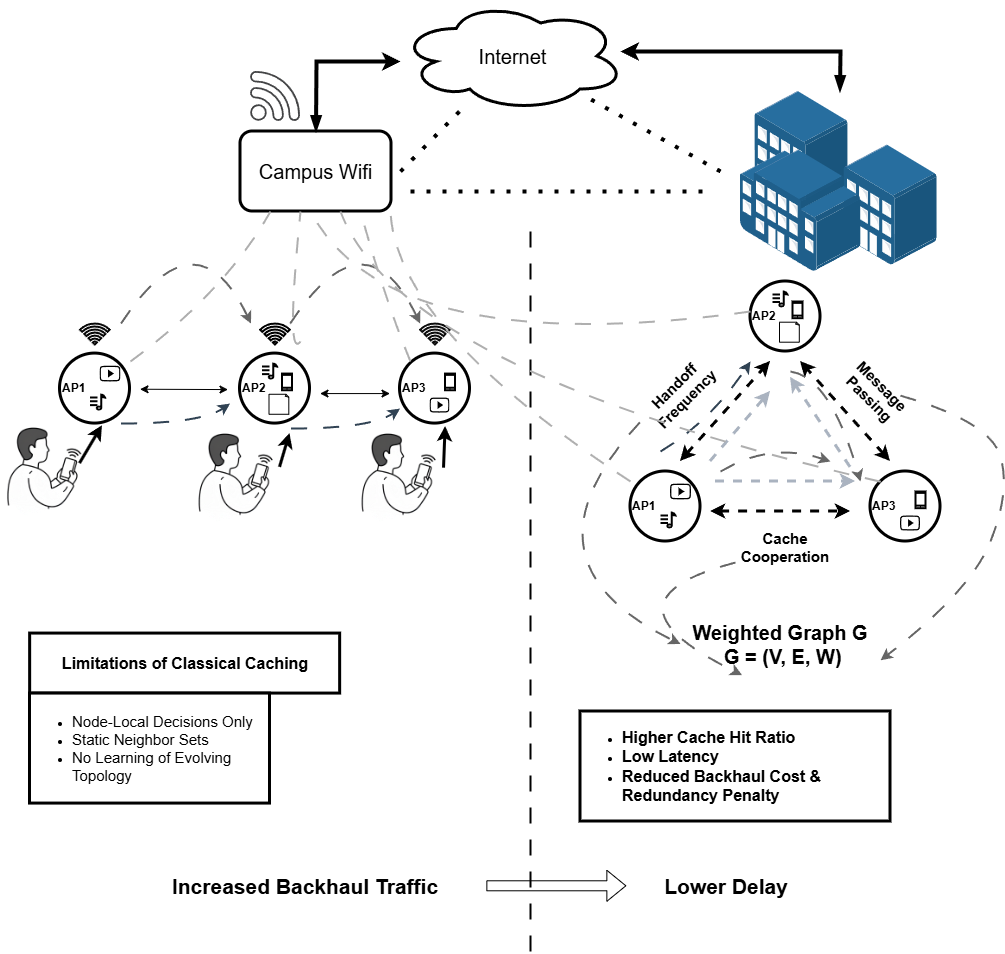
\includegraphics[width=0.8\textwidth]{iot_project.drawio.png}
    \caption{Traditional Caching vs Cooperative Caching}
    \label{fig}
    \vspace{1\baselineskip}
\end{figure}

Edge caching is a key mechanism for reducing latency and backhaul congestion in IoT-driven edge networks. Such systems consist of distributed edge nodes (e.g., access points or gateways) that serve mobile users under limited storage capacity. Due to user mobility and spatial locality, content requests observed at different edge nodes are correlated rather than independent.

In practice, these correlations induce a structured interaction topology among edge nodes. We model the edge network as a weighted graph:

\[
G = (V, E, W),
\]

where $V = \{v_1, \dots, v_N\}$ denotes the set of edge nodes, and $W(i,j)$ quantifies the strength of mobility-induced interaction between nodes $v_i$ and $v_j$, derived from aggregated user handoff patterns.

Each node $v_i$ maintains a cache $\mathcal{K}_i \subseteq \mathcal{C}$ subject to capacity constraint $C_i$. Content requests are generated according to synthetic demand distributions designed to reflect realistic workload characteristics, including global popularity skew and spatial locality across nodes.

Existing caching strategies typically operate in one of two ways:

\begin{itemize}
    \item \textbf{Node-local policies}, which update $\mathcal{K}_i$ based solely on local request history,
    \item \textbf{Heuristic cooperative policies}, which incorporate limited neighbor information using predefined neighborhood structures.
\end{itemize}

However, these approaches do not explicitly leverage the mobility-induced topology $G$ when determining cache placement decisions. As a result, they often lead to redundant content replication, inefficient cache utilization, and increased backhaul traffic.

We therefore define the topology-aware cooperative caching problem as follows:

\textbf{Given:}
\begin{itemize}
    \item A static mobility-derived graph $G$,
    \item Synthetic request streams generated per node,
    \item Cache capacity constraints $\{C_i\}$,
\end{itemize}

\textbf{Find a joint caching policy}

\[
\pi : (G, \{\mathcal{K}_i\}) \rightarrow \{\mathcal{K}_i'\},
\]

that determines cache placement across nodes to maximize overall system utility, measured in terms of:

\begin{itemize}
    \item Cache hit ratio,
    \item Latency reduction,
    \item Backhaul traffic minimization,
    \item Reduction of redundant replication across neighboring nodes.
\end{itemize}

The central research question is whether explicitly incorporating the mobility-derived topology $G$ into the caching policy $\pi$ yields measurable performance improvements over node-local and heuristic cooperative approaches.

% \section{Problem Statement}

We consider a distributed edge caching system in which a set of edge nodes, such as WiFi access points, serve content requests generated by mobile users. Each node has limited cache capacity and may satisfy a request in one of three ways: by serving the content from its own local cache, by retrieving it from another node in the network, or by fetching it from the origin server. Since users move between nodes, request patterns observed at different nodes are not independent. Instead, mobility induces structural correlations among nodes, which makes cache placement a network-level decision problem rather than a purely local one.

We represent the system as a weighted graph
\[
G = (V, E, W),
\]
where \(V\) is the set of edge nodes, \(E\) is the set of connectivity relations, and \(W = \{w_{ij}\}\) denotes mobility-induced interaction strengths. Intuitively, a larger value of \(w_{ij}\) indicates that nodes \(i\) and \(j\) are more strongly related, for example through frequent user handoffs or overlapping mobility patterns.

The objective is to design a topology-aware cooperative caching strategy that improves content accessibility while controlling replication overhead and reducing unnecessary redundancy across strongly related nodes.

\subsection{Subproblems}

\subsubsection{Demand Modeling under Partial Observability}
The available mobility trace provides user--node association information but does not include content-level request logs. Therefore, the request process must be modeled synthetically. This creates a demand estimation problem: the workload should preserve realistic properties such as skewed popularity, spatial locality, and temporal variation, while remaining simple enough for controlled evaluation.

\subsubsection{Cooperative Cache Placement}
Cache placement decisions are coupled across nodes. If each node caches content independently, neighboring nodes may store the same items and waste storage. If all decisions are fully centralized, the coordination overhead becomes impractical. The system therefore requires a cooperative placement strategy that uses topology information without assuming unrealistic global synchronization.

\subsubsection{Access--Replication Tradeoff}
Replicating content across multiple nodes improves accessibility and lowers response time, but it also consumes storage and incurs maintenance or update cost. An effective strategy must balance the gain in access efficiency against the cost of replication.

\subsubsection{Topology-Aware Redundancy Control}
Nodes with strong interaction weights tend to experience correlated demand. Storing identical content at all such nodes may reduce effective cache diversity. A useful caching policy should therefore discourage redundant replication among strongly connected nodes while preserving accessibility.

\subsection{Problem Formulation}

We model the edge network as a weighted graph \(G = (V, E, W)\), where \(V\) is the set of edge nodes, \(E\) denotes connectivity between nodes, and \(w_{ij}\) represents the strength of mobility-induced interaction between nodes \(i\) and \(j\). Stronger edge weights indicate higher mobility correlation and therefore higher potential for cooperative caching.

Let \(\mathcal{C}\) denote the content catalog. For each node \(i \in V\) and content \(c \in \mathcal{C}\), we define a binary placement variable:
\[
x_{i,c} =
\begin{cases}
1, & \text{if content } c \text{ is cached at node } i,\\
0, & \text{otherwise.}
\end{cases}
\]

Let \(P_{i,c}\) denote the probability that node \(i\) requests content \(c\), and let \(f_c\) denote the replication-related cost of content \(c\), which may reflect update frequency, storage burden, or a combined maintenance factor.

Let \(d(i,j)\) be the shortest-path distance between nodes \(i\) and \(j\), and let \(L(i,j)\) denote the latency of retrieving content from node \(j\) to node \(i\). We assume that \(L(i,j)\) is non-decreasing with graph distance. Let \(L_{\text{local}}\) denote the latency of serving content from the local cache, and let \(L_{\text{origin}}\) denote the latency of fetching it from the origin server.

To simplify the notation, we define the best non-local retrieval latency for content \(c\) at node \(i\) under placement \(x\) as
\[
A_{i,c}(x)
=
\min\!\left(
L_{\text{origin}},
\;
\min_{\substack{j \in V \\ j \neq i \\ x_{j,c}=1}} L(i,j)
\right).
\]
If no other node caches content \(c\), then \(A_{i,c}(x)=L_{\text{origin}}\).

The expected access cost is defined as
\[
C_{\text{access}}(x)
=
\sum_{i \in V}\sum_{c \in \mathcal{C}}
P_{i,c}
\left[
x_{i,c}L_{\text{local}}
+
(1-x_{i,c})A_{i,c}(x)
\right].
\]
This term captures the average latency experienced by requests under the current cache placement.

The total replication cost is given by
\[
C_{\text{rep}}(x)
=
\sum_{i \in V}\sum_{c \in \mathcal{C}}
\gamma f_c x_{i,c},
\]
where \(\gamma > 0\) scales the importance of replication overhead. This term penalizes storing too many replicas, especially for contents that are expensive to maintain or update.

To discourage unnecessary duplication among strongly related nodes, we define the topology-aware redundancy term:
\[
C_{\text{red}}(x)
=
\sum_{c \in \mathcal{C}}
\sum_{\substack{i,j \in V \\ i<j}}
w_{ij}\,x_{i,c}x_{j,c}.
\]
This term becomes large when the same content is placed at multiple nodes that have strong mobility-induced interaction, thus reducing effective cache diversity.

The overall objective is to jointly minimize access cost, replication cost, and redundancy. We formulate the topology-aware cooperative caching problem as
\[
\min_{x}
\quad
C_{\text{access}}(x)
+
\lambda C_{\text{rep}}(x)
+
\beta C_{\text{red}}(x),
\]
where \(\lambda > 0\) and \(\beta > 0\) are tradeoff parameters. Specifically, \(\lambda\) controls the relative penalty assigned to replication overhead, while \(\beta\) controls the strength of redundancy suppression among strongly connected nodes.

This formulation captures the central design tradeoff of the system. A placement that aggressively replicates content may reduce access latency but will incur larger replication and redundancy costs. Conversely, a placement that overly avoids replication may reduce storage overhead but increase access latency due to more frequent remote retrievals. The optimal caching policy therefore balances these competing effects under storage and communication constraints.

\subsection{Constraints}

The optimization problem is subject to several practical constraints.

\paragraph{Cache Capacity Constraint.}
Each edge node has limited storage and therefore cannot cache the entire content catalog. If \(K_i\) denotes the cache capacity of node \(i\), then
\[
\sum_{c \in \mathcal{C}} x_{i,c} \le K_i,
\qquad \forall i \in V.
\]

\paragraph{Binary Placement Constraint.}
Caching is a discrete decision, so
\[
x_{i,c} \in \{0,1\},
\qquad \forall i \in V,\; \forall c \in \mathcal{C}.
\]

\paragraph{Latency Ordering Constraint.}
Serving content locally is assumed to be cheaper than retrieving it from another node, and origin access is the most expensive:
\[
L_{\text{local}} < L(i,j) \le L_{\text{origin}},
\qquad \forall i,j \in V,\; i \neq j.
\]

\paragraph{Topology-Dependent Retrieval Constraint.}
Inter-node retrieval cost depends on the graph structure through \(L(i,j)\), which is determined by path distance and connectivity conditions. This ensures that the topology directly influences the cost of cooperative content access.


\begin{figure}[t]
\centering
\begin{tikzpicture}[
    node distance=2.0cm and 2.4cm,
    ap/.style={
        draw,
        rounded corners,
        minimum width=1.8cm,
        minimum height=1.0cm,
        align=center,
        font=\small
    },
    cache/.style={
        draw,
        rectangle split,
        rectangle split parts=2,
        rounded corners,
        minimum width=1.8cm,
        minimum height=0.9cm,
        align=center,
        font=\scriptsize
    },
    origin/.style={
        draw,
        ellipse,
        minimum width=2.2cm,
        minimum height=1cm,
        align=center,
        font=\small
    },
    edge/.style={thick},
    req/.style={-{Latex[length=2.5mm]}, thick},
    coop/.style={-{Latex[length=2.5mm]}, dashed, thick},
    note/.style={font=\scriptsize, align=center}
]

% Nodes
\node[cache] (ap1) {AP1 \nodepart{second} Cache: $c_1,c_3$};
\node[cache, right=of ap1] (ap2) {AP2 \nodepart{second} Cache: $c_2,c_4$};
\node[cache, below=of ap1] (ap3) {AP3 \nodepart{second} Cache: $c_1,c_5$};
\node[cache, below=of ap2] (ap4) {AP4 \nodepart{second} Cache: $c_3,c_6$};

% Origin
\node[origin, right=3.2cm of ap2] (origin) {Origin Server};

% Mobility-induced graph edges
\draw[edge] (ap1) -- node[above, font=\scriptsize] {$w_{12}$} (ap2);
\draw[edge] (ap1) -- node[left, font=\scriptsize] {$w_{13}$} (ap3);
\draw[edge] (ap2) -- node[right, font=\scriptsize] {$w_{24}$} (ap4);
\draw[edge] (ap3) -- node[below, font=\scriptsize] {$w_{34}$} (ap4);
\draw[edge] (ap1) -- node[sloped, above, font=\scriptsize] {$w_{14}$} (ap4);

% Request arrows
\draw[req] ([xshift=-0.9cm]ap1.west) -- node[above, font=\scriptsize] {request $c_2$} (ap1.west);

% Cooperative retrieval
\draw[coop, bend left=15] (ap1.north east) to node[above, font=\scriptsize] {neighbor fetch} (ap2.north west);

% Origin fetch
\draw[req, bend left=10] (ap3.east) to node[above, font=\scriptsize] {origin fetch} (origin.west);

% Labels / notes
\node[note, below=0.3cm of ap3] {Local hit if content is in \\ node cache};
\node[note, below=0.3cm of ap4] {Otherwise retrieve from \\ another node or origin};

\end{tikzpicture}
\caption{Topology-aware cooperative caching problem. Each edge node has limited cache capacity and participates in a mobility-induced graph. A request may be served locally, cooperatively from another node, or from the origin server, depending on cache placement and graph connectivity.}
\label{fig:problem_model}
\end{figure}
\section{Problem Statement}

We consider a distributed edge caching system in which a set of edge nodes collaboratively serve content requests generated by mobile users. Each node has limited cache capacity and may satisfy a request either locally, by retrieving the content from another node in the network, or by accessing the origin server. Since users move across nodes, the system exhibits mobility-induced correlations: nodes that frequently exchange users tend to observe related access patterns and may benefit from coordinated caching decisions.

We represent the system by a weighted graph \(G=(V,E,W)\), where \(V\) is the set of edge nodes, \(E\) is the set of connectivity relations, and \(W=\{w_{ij}\}\) captures mobility-induced interaction strength between nodes. Larger values of \(w_{ij}\) indicate stronger relationships, such as frequent handoffs or persistent overlap in user movement. Unlike classical caching systems in which each node is optimized independently, this setting gives rise to a coupled decision problem: content placement at one node affects accessibility, redundancy, and traffic at other nodes.

In practice, the network topology is not perfectly stable. Nodes may be added or removed due to mobility, intermittent availability, failures, or deployment changes. To model this uncertainty, we consider a perturbed graph \(\tilde{G}=(\tilde{V},\tilde{E},\tilde{W})\) sampled from a perturbation process \(\mathcal{P}(G)\), which captures random node arrivals and departures. A useful caching policy must therefore remain effective not only for the nominal graph \(G\), but also on average under such perturbations.

\subsection{Subproblems}

\subsubsection{Demand Modeling under Partial Observability}
The mobility trace provides user--node association information, but it does not include content-level request logs. As a result, demand must be synthesized while preserving realistic characteristics such as skewed popularity, spatial locality, and temporal variability. This creates a demand modeling problem: the request process should be realistic enough to support meaningful caching evaluation, yet controlled enough to avoid introducing artificial bias.

\subsubsection{Topology-Aware Cooperative Placement}
Caching decisions are coupled through the graph structure. If each node optimizes only for its own local demand, neighboring nodes may store the same content repeatedly, wasting cache space. On the other hand, fully centralized global optimization is costly and often unrealistic in distributed systems. The challenge is to exploit topology-aware cooperation without requiring complete global synchronization.

\subsubsection{Access--Replication Tradeoff}
Replicating content across more nodes improves accessibility and lowers retrieval latency, but it also consumes storage and incurs maintenance overhead. A good caching strategy must therefore balance the gain in access efficiency against the cost of storing and maintaining replicas.

\subsubsection{Relocation under Topology Perturbation}
When the topology changes due to node additions or removals, a previously efficient cache placement may become suboptimal. The system should be able to relocate cached content to adapt to perturbations, but relocation itself incurs communication and replacement cost. Thus, the policy must balance robustness against instability.

\subsection{Formal Problem Formulation}

Let \(\mathcal{C}\) denote the content catalog. For each node \(i \in \tilde{V}\) and content item \(c \in \mathcal{C}\), define the binary placement variable
\[
x_{i,c} =
\begin{cases}
1, & \text{if content } c \text{ is cached at node } i,\\
0, & \text{otherwise.}
\end{cases}
\]

Let \(x^{0}_{i,c}\) denote the initial cache state before perturbation. Let \(P_{i,c}\) denote the probability that node \(i\) requests content \(c\), and let \(f_c\) denote the replication-related cost of content \(c\), which may reflect update frequency, storage burden, or a combined maintenance factor.

Let \(d(i,j)\) be the shortest-path distance between nodes \(i\) and \(j\) in the perturbed graph \(\tilde{G}\), and let \(L(i,j)\) denote the latency of retrieving content from node \(j\) to node \(i\). We assume that \(L(i,j)\) is a non-decreasing function of graph distance. Let \(L_{\text{local}}\) denote the latency of serving content from the local cache, and let \(L_{\text{origin}}\) denote the latency of retrieving content from the origin server.

To simplify notation, define the best non-local retrieval latency for content \(c\) at node \(i\) under placement \(x\) and perturbed topology \(\tilde{G}\) as
\[
A_{i,c}(x,\tilde{G})
=
\min\!\left(
L_{\text{origin}},
\;
\min_{\substack{j \in \tilde{V} \\ j \neq i \\ x_{j,c}=1}} L(i,j)
\right).
\]
If no other node stores content \(c\), then \(A_{i,c}(x,\tilde{G}) = L_{\text{origin}}\).

The expected access cost is
\[
C_{\text{access}}(x,\tilde{G})
=
\sum_{i \in \tilde{V}} \sum_{c \in \mathcal{C}}
P_{i,c}
\left[
x_{i,c} L_{\text{local}}
+
(1-x_{i,c}) A_{i,c}(x,\tilde{G})
\right].
\]

The replication cost is
\[
C_{\text{rep}}(x,\tilde{G})
=
\sum_{i \in \tilde{V}} \sum_{c \in \mathcal{C}}
\gamma f_c x_{i,c},
\]
where \(\gamma > 0\) scales the importance of replication overhead.

To discourage redundant placement among strongly related nodes, we define the topology-aware redundancy penalty
\[
C_{\text{red}}(x,\tilde{G})
=
\sum_{c \in \mathcal{C}}
\sum_{\substack{i,j \in \tilde{V} \\ i<j}}
\tilde{w}_{ij}\,x_{i,c}x_{j,c}.
\]

To capture the cost of adapting the cache after perturbation, we define the relocation cost
\[
C_{\text{rel}}(x,x^{0})
=
\sum_{i \in \tilde{V}} \sum_{c \in \mathcal{C}}
\delta_c \, |x_{i,c} - x^{0}_{i,c}|,
\]
where \(\delta_c\) denotes the cost of adding or removing content \(c\) at a node.

The topology-aware cooperative caching problem is therefore formulated as the following stochastic optimization problem:
\[
\min_{x}
\;
\mathbb{E}_{\tilde{G} \sim \mathcal{P}(G)}
\left[
C_{\text{access}}(x,\tilde{G})
+ \lambda C_{\text{rep}}(x,\tilde{G})
+ \beta C_{\text{red}}(x,\tilde{G})
+ \mu C_{\text{rel}}(x,x^{0})
\right],
\]
where \(\lambda > 0\), \(\beta > 0\), and \(\mu > 0\) control the tradeoff between access efficiency, replication overhead, redundancy reduction, and relocation stability.

This objective captures the central design challenge of the system. Aggressive replication can reduce latency but increases replication and redundancy cost. Conservative placement may reduce overhead but increase expensive remote retrievals. Frequent relocation may adapt well to perturbations but can incur substantial update cost. The desired policy is therefore one that minimizes expected overall cost under random topology perturbations.

\subsection{Constraints}

The optimization problem is subject to the following practical constraints.

\paragraph{Cache Capacity Constraint.}
Each node has limited storage and therefore cannot cache the entire catalog. If \(K_i\) denotes the cache capacity of node \(i\), then the total size or number of cached items must remain within its budget:
\[
\sum_{c \in \mathcal{C}} x_{i,c} \le K_i,
\qquad \forall i \in \tilde{V}.
\]
This ensures that the solution is feasible under node-level storage limitations.

\paragraph{Binary Placement Constraint.}
Caching is a discrete decision: an item is either stored at a node or it is not. Therefore,
\[
x_{i,c} \in \{0,1\},
\qquad \forall i \in \tilde{V},\; \forall c \in \mathcal{C}.
\]
This makes the placement problem combinatorial.

\paragraph{Latency Ordering Constraint.}
The system assumes a natural service hierarchy: local cache access is cheapest, inter-node retrieval is more expensive, and origin retrieval is most expensive:
\[
L_{\text{local}} < L(i,j) \le L_{\text{origin}},
\qquad \forall i,j \in \tilde{V},\; i \neq j.
\]
This reflects the fact that cooperation is beneficial but not free.

\paragraph{Perturbation Feasibility Constraint.}
Cache placement after perturbation is only defined on nodes that remain present in \(\tilde{V}\). Newly added nodes may begin with empty cache state, while removed nodes cannot participate in storage or retrieval. This ensures that placement and relocation decisions are consistent with the realized perturbed topology.

\paragraph{Topology-Dependent Communication Constraint.}
Inter-node retrieval cost depends on the perturbed graph structure through \(L(i,j)\). Thus, cooperation is not assumed to be globally uniform or free; it is mediated by graph connectivity and path cost. This ensures that the topology plays a direct and meaningful role in the optimization problem.
\section{Dataset}

The intended real-world mobility source is the CRAWDAD Dartmouth Campus Wi-Fi dataset. The current official Dartmouth author page describes the 2009 release as a dataset containing syslog, SNMP, and tcpdump data for more than five years, covering more than 450 access points and several thousand users at Dartmouth College \cite{kotz_dartmouth_campus_2009}. Earlier Dartmouth releases and papers report detailed AP association and handoff traces collected between 2001 and 2004, and these traces have been widely used for campus-scale WLAN mobility modeling \cite{Kotz2004Dartmouth,kim2005mobility_wifi_ap}. The dataset is appropriate for this project because edge nodes can be represented by access points, and user movement among APs naturally induces the cooperative caching topology.

\subsection{Access and Reproducibility}

The implementation includes \texttt{scripts/download\_dataset.py}, which records official dataset landing pages and writes a local access note in \texttt{data/raw/dartmouth\_access/ACCESS\_NOTE.txt}. During this run, legacy direct CRAWDAD download paths for the movement archive returned HTTP 404, while the official author page points to IEEE DataPort. Because raw archive download may require browser interaction, account access, or DataPort terms acceptance, the repository also provides a deterministic trace-compatible fallback generator. This fallback is not presented as the original Dartmouth data; it is used to make the full pipeline executable when the raw trace is unavailable locally.

The fallback trace is saved as \texttt{data/raw/dartmouth\_movement.csv} with columns \texttt{user\_id}, \texttt{timestamp}, and \texttt{ap}. A sidecar metadata file marks the trace as synthetic. The generated trace preserves the operational structure needed by the methodology: users repeatedly associate with named APs, transition among nearby AP clusters, occasionally leave the network through an \texttt{OFF} state, and produce ordered AP sequences from which handoffs can be extracted.

\subsection{Preprocessing}

The preprocessing stage accepts any movement trace with the same three-column format. Records are sorted by user and timestamp. \texttt{OFF} intervals are removed before graph construction because they represent absence from the WLAN rather than a cache-serving edge node. Consecutive repeated AP observations are collapsed implicitly: only transitions where the AP changes contribute to the handoff count. For a user sequence
\[
i_1, i_2, \ldots, i_T,
\]
each adjacent transition \(i_t \rightarrow i_{t+1}\), where \(i_t \neq i_{t+1}\), increments a handoff counter \(H_{i_t,i_{t+1}}\). This follows WLAN mobility work that models mobility at the AP association level rather than requiring exact physical paths \cite{kim2005mobility_wifi_ap,shin2004neighbor_graphs}.

For computational tractability in the local experiment, the implementation selects the most active APs and keeps the largest connected component. The final run used 20 AP nodes and 190 weighted edges from 25,600 generated association records. This graph is dense enough to support cooperative retrieval and small enough for repeated greedy and DQN evaluation.

\begin{table}[t]
\centering
\caption{Dataset and graph statistics for the reproducible run included with the repository.}
\label{tab:dataset_stats}
\begin{tabular}{lr}
\toprule
Property & Value \\
\midrule
Movement records & 25,600 \\
Selected AP nodes & 20 \\
Weighted mobility edges & 190 \\
Content catalog size & 48 \\
Cache capacity per node & 5 objects \\
Zipf skew parameter \(\alpha\) & 0.85 \\
Spatial locality multiplier & 2.8 \\
Synthetic fallback used & Yes \\
\bottomrule
\end{tabular}
\end{table}

\subsection{Synthetic Content Demand}

The Dartmouth movement traces do not contain content request logs. Therefore, content demand is synthesized while preserving two common properties of edge workloads: skewed content popularity and spatial locality. Global content popularity follows a Zipf distribution, a standard model for web and content caching workloads \cite{breslau1999zipf,Podlipnig2003}. For catalog rank \(r\), global popularity is
\[
p_r = \frac{r^{-\alpha}}{\sum_{k=1}^{M} k^{-\alpha}},
\]
where \(M\) is the catalog size and \(\alpha\) controls skew. Node-specific demand then applies a locality multiplier to content groups associated with the node's AP cluster and renormalizes the distribution. This makes nearby APs partially correlated while still retaining global popularity pressure, which is important for evaluating both redundancy and diversity.

The demand model is intentionally controlled. Since real content requests are unavailable, every result should be interpreted as trace-structured simulation rather than direct measurement of Dartmouth user content preferences. The advantage of this design is that cache policies can be compared under identical seeds, catalog sizes, cache capacities, and perturbation rates.

% \section{Proposed Methodology for Phase 2}

We propose a systematic approach to learn topology-aware caching policies for IoT edge networks, which we plan to implement in phase 2.
Our proposed methodology consists of five stages: (i) graph construction from mobility traces, (ii) workload modeling, (iii) trace-driven simulation, (iv) baseline policy implementation, and (v) topology-aware cooperative caching design and evaluation.

\subsection{Graph Construction from Mobility Traces}
We utilize large-scale Wi-Fi association logs to construct a mobility-driven edge network graph. Each access point (AP) is modeled as an edge node (cache). Inter-node relationships are derived from user handoff patterns: if a device transitions from AP $i$ to AP $j$, we add (or increment) an edge $(i,j)$. The resulting weighted graph is:
\[
G = (V, E, W),
\]
where $V$ is the set of APs, $E$ is the set of edges induced by handoffs, and $W$ contains edge weights proportional to handoff frequency (optionally normalized). This graph captures topological dependencies induced by real mobility.

\subsection{Workload Modeling}
Since mobility datasets typically do not include content identifiers, we generate a synthetic but realistic request workload layered on the mobility trace. Requests follow:
\begin{itemize}
    \item Zipf-like global popularity,
    \item Spatial locality (node-specific preference skews),
    \item Temporal dynamics (popularity drift and burstiness).
\end{itemize}
Each request event is represented as:
\[
r_k = (t_k, v_k, c_k, s_k),
\]
where $t_k$ is the timestamp, $v_k \in V$ is the edge node serving the device at time $t_k$, $c_k$ is the content identifier, and $s_k$ is the content size.

\subsection{Trace-Driven Simulation from the Dataset}
We perform a discrete-event, trace-driven simulation in which the mobility trace determines \emph{where} requests arrive and the workload model determines \emph{what} is requested.

\paragraph{Mapping users to edge nodes.}
For each device $u$ and request timestamp $t_k$, we determine the associated AP by selecting the association interval $(\text{start}, \text{end})$ such that $\text{start} \le t_k \le \text{end}$. This yields $v_k$, the edge node receiving the request. The simulation advances in chronological order of events.

\paragraph{Service model.}
For each request $(t_k, v_k, c_k, s_k)$, the simulator applies a fixed service procedure shared across all policies:
\begin{enumerate}
    \item \textbf{Local cache lookup:} if $c_k$ is stored at node $v_k$, the request is a local hit.
    \item \textbf{Neighbor lookup (cooperation):} otherwise, the simulator checks one-hop neighbors $\mathcal{N}(v_k)$ (or two-hop, if configured). If a neighbor stores $c_k$, the request is served from that neighbor (neighbor hit).
    \item \textbf{Origin fetch:} if no cache contains $c_k$ within the search radius, the content is fetched from the origin/cloud (backhaul miss).
\end{enumerate}

\paragraph{Latency and cost accounting.}
We associate latency/cost with each serving source:
\begin{itemize}
    \item Local hit: $L_{\text{local}}$,
    \item Neighbor hit: $L_{\text{nbr}}(v_k,j)$ derived from graph distance or edge weight (e.g., proportional to handoff weight or a configured link-latency model),
    \item Origin fetch: $L_{\text{origin}}$ and backhaul traffic increment by $s_k$.
\end{itemize}
This enables evaluation beyond hit ratio, including latency and backhaul usage.

\paragraph{Cache updates and decision cadence.}
Caching policies may update:
\begin{itemize}
    \item \textbf{Per-request:} update cache state after each event (typical for LRU/LFU), or
    \item \textbf{Windowed:} update caches every fixed interval $\Delta$ (e.g., 1--10 minutes), which is suitable for learning-based policies.
\end{itemize}
For windowed updates, we aggregate per-node demand statistics within each window to form features and compute cache placement for the next window.

\subsection{Baseline Caching Policies}
We implement representative baselines for comparison:
\begin{itemize}
    \item \textbf{Node-local caching:} LRU, LFU,
    \item \textbf{Heuristic cooperative caching:} neighbor-assisted caching (serve from neighbor if available; optional diversity heuristic to reduce redundancy),
    \item \textbf{Local learning-based caching:} per-node popularity prediction (e.g., time-series model) followed by top-$K$ placement.
\end{itemize}

\subsection{Topology-Aware Cooperative Caching via Graph Learning}
We propose a topology-aware framework where caching decisions are learned jointly using the graph $G$.

Let $x_i$ denote node features for edge node $i$ (recent demand statistics, cache occupancy, neighbor hit rates, etc.). A graph learning model computes node embeddings:
\[
h_i = \mathrm{GNN}(G, X)_i,
\]
where $X = \{x_i\}_{i \in V}$. For content $c$, we define a cache score:
\[
s_{i,c} = f(h_i, e_c),
\]
where $e_c$ is a content embedding and $f(\cdot)$ is a scoring function (e.g., inner product). Node $i$ caches the top-$K$ items ranked by $s_{i,c}$ subject to capacity constraints. This enables decentralized execution while incorporating topological context through learned message passing.

\subsection{Evaluation Metrics}
We evaluate all policies under identical trace-driven simulation settings using:
\begin{itemize}
    \item Cache Hit Ratio (CHR) and Neighbor Hit Ratio,
    \item Average latency (and tail latency, if reported),
    \item Backhaul traffic volume (bytes fetched from origin),
    \item Redundancy/diversity metrics across caches (replication rate, unique cached items),
    \item Scalability with respect to number of nodes and cache capacity.
\end{itemize}
We conduct sensitivity analyses over mobility intensity, cache size, cooperation radius, and demand drift to characterize when topology-aware policies provide the largest benefit.

% \section{Proposed Methodology for Phase 2}

In Phase 2, we implement and evaluate topology-aware cooperative caching over a mobility-derived static graph using synthetic workloads. The methodology consists of four main components: (i) graph construction, (ii) workload generation and trace-driven simulation, (iii) baseline implementation, and (iv) topology-aware policy design.

\subsection{Graph Construction}

We construct a static edge network graph from Wi-Fi mobility traces. Each access point (AP) is modeled as a node in the network. If users transition between AP $i$ and AP $j$, we increment the edge weight between them. After aggregating transitions over the dataset, we obtain:

\[
G = (V, E, W),
\]

where $W(i,j)$ reflects the normalized frequency of user handoffs. This graph encodes mobility-induced structural relationships among edge nodes.

\subsection{Synthetic Workload Generation}

Since mobility traces do not include content identifiers, we generate synthetic request streams for each node. The workload incorporates:

\begin{itemize}
    \item Zipf-like global popularity distribution,
    \item Spatial locality (node-specific demand skew),
    \item Temporal variation in request rates.
\end{itemize}

Each request is represented as:
\[
r_k = (t_k, v_k, c_k, s_k),
\]
where $v_k$ is the serving node determined by mobility association, $c_k$ is the requested content, and $s_k$ is the content size.

\subsection{Trace-Driven Simulation}

We perform a discrete-event simulation in chronological order of requests. For each request:

\begin{enumerate}
    \item If content is in the local cache, record a local hit.
    \item Otherwise, check neighboring nodes within a predefined cooperation radius.
    \item If unavailable, fetch from the origin and record backhaul cost.
\end{enumerate}

Latency and traffic metrics are recorded for evaluation. Cache updates occur either per request (for LRU/LFU) or at fixed time windows (for learning-based methods).

\subsection{Baseline Policies}

We implement three baseline categories:

\begin{itemize}
    \item Node-local caching (LRU, LFU),
    \item Heuristic cooperative caching,
    \item Local popularity-based learning.
\end{itemize}

\subsection{Topology-Aware Cooperative Policy}

We design a graph-based policy that jointly determines cache placement using structural information from $G$. Given node features $x_i$, a graph learning model computes node representations:

\[
h_i = \mathrm{GNN}(G, X)_i.
\]

For each content $c$, a scoring function $s_{i,c} = f(h_i, e_c)$ determines its priority at node $i$. Each node caches the top-$K$ items under capacity constraints. This approach enables decentralized yet topology-aware coordination.

\subsection{Evaluation}

All methods are evaluated under identical simulation settings using:

\begin{itemize}
    \item Cache Hit Ratio (CHR),
    \item Average latency,
    \item Backhaul traffic volume,
    \item Redundancy and cache diversity metrics,
    \item Scalability with respect to network size and cache capacity.
\end{itemize}

\section{Methodology}

\subsection{Overview}

We propose a two-stage topology-aware cooperative caching framework that combines a greedy initialization procedure with a deep reinforcement learning (DRL) refinement phase. The greedy stage provides a fast, interpretable, and cost-aware initial placement, while the DRL stage refines this placement under random topology perturbations. This hybrid design is motivated by two considerations. First, the caching problem is combinatorial and difficult to solve exactly at scale. Second, directly training a DRL agent over the full placement space is inefficient without a strong initialization.

The complete pipeline consists of the following steps:
\begin{enumerate}
    \item Construct a mobility-derived nominal graph \(G=(V,E,W)\) from the dataset.
    \item Generate synthetic request probabilities \(P_{i,c}\) over the content catalog.
    \item Create random perturbed graph instances \(\tilde{G} \sim \mathcal{P}(G)\) through node addition and removal.
    \item Compute an initial placement using a topology-aware greedy algorithm.
    \item Refine the placement using DRL, with reward defined by the negative expected total cost.
\end{enumerate}

\begin{figure}[t]
\centering
\begin{tikzpicture}[
    node distance=1.35cm,
    block/.style={draw, rounded corners, minimum width=3.2cm, minimum height=0.85cm, align=center},
    arrow/.style={-{Latex[length=2.5mm]}, thick}
]
\node[block] (data) {Mobility Trace};
\node[block, below=of data] (graph) {Nominal Graph Construction};
\node[block, below=of graph] (demand) {Synthetic Demand Generation};
\node[block, below=of demand] (perturb) {Topology Perturbation Sampler};
\node[block, below left=0.8cm and 1.8cm of perturb] (greedy) {Greedy Initialization};
\node[block, below right=0.8cm and 1.8cm of perturb] (drl) {DRL Refinement};
\node[block, below=1.6cm of perturb] (final) {Robust Cache Placement};

\draw[arrow] (data) -- (graph);
\draw[arrow] (graph) -- (demand);
\draw[arrow] (demand) -- (perturb);
\draw[arrow] (perturb) -- (greedy);
\draw[arrow] (perturb) -- (drl);
\draw[arrow] (greedy) -- (final);
\draw[arrow] (drl) -- (final);
\end{tikzpicture}
\caption{Methodology pipeline: the system builds a nominal mobility graph, generates demand and perturbations, computes a greedy initial placement, and then refines it through DRL.}
\label{fig:method_pipeline}
\end{figure}

\subsection{Graph Construction and Perturbation Model}

We first construct a nominal weighted graph \(G=(V,E,W)\) from user handoff traces. For each pair of nodes \(i,j \in V\), let \(H_{ij}\) denote the number of observed handoffs from \(i\) to \(j\). We define the normalized interaction weight as
\[
w_{ij} = \frac{H_{ij}}{\sum_{k} H_{ik}}.
\]
Edges with negligible transition frequency may be removed by thresholding.

To model topology uncertainty, we define a perturbation process \(\mathcal{P}(G)\) that generates a perturbed graph \(\tilde{G} = (\tilde{V}, \tilde{E}, \tilde{W})\) by randomly removing and adding nodes. When a node is removed, all incident edges are deleted. When a node is added, its incident edges are inferred from the mobility model or sampled from historical transition statistics. This perturbation model is used both during greedy evaluation and DRL training.

\subsection{Synthetic Demand Model}

Since the dataset does not include content requests, demand is generated synthetically. Let \(\mathcal{C}\) be the content catalog. Global content popularity follows a Zipf distribution:
\[
P(c) = \frac{c^{-\alpha}}{\sum_{m=1}^{|\mathcal{C}|} m^{-\alpha}},
\]
where \(\alpha > 0\) controls the skewness.

To capture spatial locality, the node-specific demand distribution is defined as
\[
P_{i,c} = \frac{\eta_{i,c} P(c)}{\sum_{c' \in \mathcal{C}} \eta_{i,c'} P(c')},
\]
where \(\eta_{i,c}\) is a locality bias factor for node \(i\) and content \(c\). This allows different nodes to prefer different subsets of the catalog.

\subsection{Cost Components}

The methodology uses the same cost terms as the problem formulation.

For a placement \(x\) on a perturbed graph \(\tilde{G}\), define the best non-local retrieval latency as
\[
A_{i,c}(x,\tilde{G})
=
\min\!\left(
L_{\text{origin}},
\;
\min_{\substack{j \in \tilde{V} \\ j \neq i \\ x_{j,c}=1}} L(i,j)
\right).
\]

Then:
\[
C_{\text{access}}(x,\tilde{G})
=
\sum_{i \in \tilde{V}} \sum_{c \in \mathcal{C}}
P_{i,c}
\left[
x_{i,c}L_{\text{local}}
+
(1-x_{i,c})A_{i,c}(x,\tilde{G})
\right],
\]
\[
C_{\text{rep}}(x,\tilde{G})
=
\sum_{i \in \tilde{V}} \sum_{c \in \mathcal{C}}
\gamma f_c x_{i,c},
\]
\[
C_{\text{red}}(x,\tilde{G})
=
\sum_{c \in \mathcal{C}}
\sum_{\substack{i,j \in \tilde{V} \\ i<j}}
\tilde{w}_{ij}x_{i,c}x_{j,c},
\]
\[
C_{\text{rel}}(x,x^0)
=
\sum_{i \in \tilde{V}} \sum_{c \in \mathcal{C}}
\delta_c |x_{i,c}-x_{i,c}^0|.
\]

The total cost under a perturbed graph is
\[
J(x,\tilde{G})
=
C_{\text{access}}(x,\tilde{G})
+
\lambda C_{\text{rep}}(x,\tilde{G})
+
\beta C_{\text{red}}(x,\tilde{G})
+
\mu C_{\text{rel}}(x,x^0).
\]

\subsection{Stage I: Greedy Topology-Aware Initialization}

The greedy stage builds the cache placement incrementally. At each step, the algorithm selects the node--content pair that gives the largest decrease in expected total cost.

Let \(x\) be the current placement. For each feasible pair \((i,c)\), define the marginal gain:
\[
\Delta(i,c \mid x)
=
\mathbb{E}_{\tilde{G} \sim \mathcal{P}(G)}
\left[
J(x,\tilde{G}) - J(x^{(i,c)},\tilde{G})
\right],
\]
where \(x^{(i,c)}\) is the placement obtained by setting \(x_{i,c}=1\), provided the capacity constraint remains satisfied.

At each iteration, the greedy algorithm chooses
\[
(i^*,c^*) = \arg\max_{(i,c)} \Delta(i,c \mid x),
\]
and updates the placement accordingly. The process stops when all caches are full or when no candidate produces positive marginal gain.

\begin{algorithm}[t]
\caption{Greedy Topology-Aware Cache Initialization}
\label{alg:greedy}
\begin{algorithmic}[1]
\Require Nominal graph \(G\), perturbation process \(\mathcal{P}(G)\), content catalog \(\mathcal{C}\), capacities \(\{K_i\}\), initial placement \(x^0\)
\Ensure Greedy cache placement \(x\)
\State Initialize \(x \gets x^0\)
\State Mark all available slots at each node
\Repeat
    \State bestGain \(\gets 0\), bestPair \(\gets \varnothing\)
    \For{each node \(i\)}
        \For{each content \(c \in \mathcal{C}\) such that \(x_{i,c}=0\) and node \(i\) has free capacity}
            \State Construct tentative placement \(x^{(i,c)}\) by setting \(x_{i,c}=1\)
            \State Estimate marginal gain
            \[
            \Delta(i,c \mid x)
            =
            \mathbb{E}_{\tilde{G} \sim \mathcal{P}(G)}
            \left[
            J(x,\tilde{G}) - J(x^{(i,c)},\tilde{G})
            \right]
            \]
            \If{\(\Delta(i,c \mid x) > \) bestGain}
                \State bestGain \(\gets \Delta(i,c \mid x)\)
                \State bestPair \(\gets (i,c)\)
            \EndIf
        \EndFor
    \EndFor
    \If{bestPair \(\neq \varnothing\)}
        \State Update \(x\) by caching \(c\) at node \(i\) for bestPair
    \EndIf
\Until{bestPair \(=\varnothing\)}
\State \Return \(x\)
\end{algorithmic}
\end{algorithm}

\subsection{Stage II: DRL-Based Refinement}

The greedy solution is then used as the initial state for DRL refinement. The DRL agent learns a placement-improvement policy under random topology perturbations.

\subsubsection{State Representation}
At each decision step, the state includes:
\begin{itemize}
    \item the current perturbed graph \(\tilde{G}\),
    \item the current cache placement \(x\),
    \item node capacities and free cache slots,
    \item node-wise demand statistics \(P_{i,c}\),
    \item graph-derived features such as degree, weighted degree, or centrality.
\end{itemize}

In the implementation, this state is encoded as a fixed-length vector formed by concatenating the binary cache placement matrix, the node-content demand matrix, and graph features for each AP. The graph features include normalized degree, normalized weighted degree, and closeness centrality computed on latency-weighted graph edges. This design keeps the model lightweight while still exposing topology information to the DQN. A graph neural network encoder would be a natural extension, but the present implementation intentionally uses explicit graph features so the pipeline remains simple enough to run locally.

\subsubsection{Action Space}
An action modifies the current placement through one of the following operations:
\begin{itemize}
    \item add content \(c\) to node \(i\),
    \item remove content \(c\) from node \(i\),
    \item swap content \(c_1\) with \(c_2\) at node \(i\),
    \item relocate content \(c\) from node \(i\) to node \(j\).
\end{itemize}
Each action must preserve feasibility under the cache capacity constraints.

For the runnable DQN experiment, actions are indexed as node-content toggle candidates. If an action adds content to a node whose cache is already full, the implementation evicts the currently cached item with the lowest local demand at that node. This converts the abstract add/remove/swap behavior into a compact discrete action space of size \(|V||\mathcal{C}|\), which is compatible with DQN and preserves the cache capacity constraint.

\subsubsection{Reward Function}
The DRL reward is defined as the negative total cost:
\[
r = -J(x,\tilde{G}).
\]
Equivalently, one may use the improvement in cost between consecutive states:
\[
r_t = J(x_t,\tilde{G}_t) - J(x_{t+1},\tilde{G}_t).
\]
This encourages the agent to find placements that reduce access cost, replication overhead, redundancy, and relocation cost simultaneously.

\subsubsection{Training Procedure}
For each training episode, a perturbed graph \(\tilde{G}\) is sampled from \(\mathcal{P}(G)\). The episode starts from the greedy placement and the agent interacts with the environment by applying cache modifications until a termination criterion is met (e.g., a maximum number of actions or no further improvement).

The DQN uses a two-layer feedforward Q-network with ReLU activations, replay buffer sampling, a target network, discount factor 0.92, learning rate 0.001, and an epsilon-greedy exploration schedule. The final run uses 85 episodes and 16 actions per episode. At inference time, candidate DQN actions are accepted only if they reduce the measured objective relative to the current placement. This acceptance rule prevents the learned refiner from degrading a strong greedy warm start and keeps relocation overhead bounded.

\begin{algorithm}[t]
\caption{DRL Refinement under Topology Perturbation}
\label{alg:drl}
\begin{algorithmic}[1]
\Require Nominal graph \(G\), perturbation process \(\mathcal{P}(G)\), greedy placement \(x^{\text{greedy}}\), replay buffer \(\mathcal{D}\)
\Ensure Refined policy \(\pi_\theta\)
\For{episode \(=1\) to \(N_{\text{episodes}}\)}
    \State Sample perturbed graph \(\tilde{G} \sim \mathcal{P}(G)\)
    \State Initialize placement \(x \gets x^{\text{greedy}}\)
    \State Construct initial state \(s_0 = (\tilde{G}, x)\)
    \For{step \(t=0\) to \(T_{\max}\)}
        \State Select action \(a_t \sim \pi_\theta(s_t)\) using \(\epsilon\)-greedy or policy sampling
        \State Apply action \(a_t\) to obtain new feasible placement \(x'\)
        \State Compute reward
        \[
        r_t = J(x,\tilde{G}) - J(x',\tilde{G})
        \]
        \State Construct next state \(s_{t+1} = (\tilde{G}, x')\)
        \State Store transition \((s_t, a_t, r_t, s_{t+1})\) in replay buffer \(\mathcal{D}\)
        \State Update policy parameters \(\theta\) using mini-batches from \(\mathcal{D}\)
        \State Set \(x \gets x'\)
        \If{termination condition is satisfied}
            \State \textbf{break}
        \EndIf
    \EndFor
\EndFor
\State \Return learned policy \(\pi_\theta\)
\end{algorithmic}
\end{algorithm}

\subsection{Greedy--DRL Hybrid Inference}

At inference time, the final placement is produced in two steps:
\begin{enumerate}
    \item compute the initial placement using Algorithm~\ref{alg:greedy};
    \item refine it using a fixed number of DRL improvement steps from Algorithm~\ref{alg:drl}.
\end{enumerate}

This hybrid strategy preserves the interpretability of the greedy approach while allowing learning-based adaptation to topology perturbations.

\begin{figure}[t]
\centering
\begin{tikzpicture}[
    node distance=1.25cm and 1.8cm,
    block/.style={draw, rounded corners, minimum width=2.8cm, minimum height=0.8cm, align=center},
    arrow/.style={-{Latex[length=2.5mm]}, thick}
]
\node[block] (start) {Initial Placement \(x^0\)};
\node[block, below=of start] (greedy) {Greedy Warm Start};
\node[block, below=of greedy] (perturb) {Sample Perturbed Graph \(\tilde{G}\)};
\node[block, below left=0.9cm and 1.8cm of perturb] (state) {State Construction};
\node[block, below right=0.9cm and 1.8cm of perturb] (action) {DRL Action};
\node[block, below=1.8cm of perturb] (update) {Placement Update};
\node[block, below=of update] (reward) {Cost / Reward Evaluation};

\draw[arrow] (start) -- (greedy);
\draw[arrow] (greedy) -- (perturb);
\draw[arrow] (perturb) -- (state);
\draw[arrow] (perturb) -- (action);
\draw[arrow] (state) -- (update);
\draw[arrow] (action) -- (update);
\draw[arrow] (update) -- (reward);
\draw[arrow] (reward.east) to[out=0,in=0,looseness=1.6] node[right] {\small feedback} (action.east);
\end{tikzpicture}
\caption{Greedy--DRL hybrid refinement. The greedy stage provides a strong initial placement; the DRL stage improves it under sampled topology perturbations.}
\label{fig:hybrid_refinement}
\end{figure}


\subsection{Evaluation Procedure}

For each final placement, we evaluate the following:
\begin{itemize}
    \item expected access cost,
    \item replication cost,
    \item redundancy penalty,
    \item relocation cost,
    \item total objective value.
\end{itemize}

These quantities are averaged over multiple perturbed graphs sampled from \(\mathcal{P}(G)\). This directly matches the stochastic objective in the problem formulation and measures the robustness of the learned caching strategy.

\subsection{Implementation Pipeline}

The complete implementation is organized as a reproducible Python package:
\begin{itemize}
    \item \texttt{src/tacc/data.py} loads a movement trace or creates the deterministic trace-compatible fallback.
    \item \texttt{src/tacc/graph.py} constructs the handoff graph, computes graph features, and samples perturbations.
    \item \texttt{src/tacc/demand.py} generates Zipf and spatial-locality demand.
    \item \texttt{src/tacc/evaluate.py} computes access cost, hit ratios, redundancy, relocation, and the full objective.
    \item \texttt{src/tacc/placement.py} implements random, local popularity, global popularity, diversified popularity, and topology-aware greedy placements.
    \item \texttt{src/tacc/rl.py} implements DQN training and accepted-action refinement.
    \item \texttt{src/tacc/reporting.py} writes report-ready LaTeX tables and figures.
    \item \texttt{scripts/run\_experiments.py} runs the full experiment and writes result files.
\end{itemize}

This structure connects the mathematical formulation to executable artifacts. Each symbol in the objective has a corresponding implementation parameter, and each reported metric is computed directly from a placement matrix, demand matrix, and perturbed graph. The code also records metadata such as graph size, random seed, fallback dataset usage, and runtime, which supports reproducibility.

\subsection{Design Rationale}

The greedy stage is responsible for global structure. It evaluates marginal node-content additions using the expected objective over sampled perturbations, so it naturally favors placements that reduce origin access while avoiding unnecessary edge-neighbor duplication. The learning stage is responsible for local improvement around the greedy solution. This division is important because the complete binary placement space is too large for naive reinforcement learning, but the neighborhood around a strong greedy solution is small enough for a compact DQN to search effectively.

The approach also separates topology-awareness from content-demand assumptions. The graph is derived from mobility handoffs, while content demand is generated from an explicit Zipf-locality model. This separation is useful because real WLAN traces often contain mobility information without application-level content identifiers. The framework can therefore accept real content logs if available, but remains usable when only mobility traces are public.





% \subsection{Discussion}

% The greedy stage provides a low-cost approximation that is easy to interpret and analyze. The DRL stage improves adaptability by learning how to respond to topology perturbations and relocation opportunities that are difficult to capture through hand-designed local rules alone. Together, the two stages produce a practical and robust cooperative caching framework.

\section{Evaluation}

\subsection{Experimental Setup}

The evaluation uses the reproducible pipeline implemented in \texttt{src/tacc/} and executed through \texttt{scripts/run\_experiments.py}. Nodes represent APs, weighted edges represent mobility handoffs, and content demand is generated using the Zipf-plus-locality model described in the Dataset section. The final experiment was executed with seed 11, 20 AP nodes, 48 content objects, cache capacity 5, Zipf parameter \(\alpha=0.85\), locality multiplier 2.8, and 12 perturbation samples per reported setting.

Topology perturbations are introduced by removing nodes with probability \(p\) and edges with probability \(p/2\), where \(p \in \{0.00,0.05,0.10,0.15\}\). After perturbation, the largest connected component is retained for evaluation. This models temporary AP unavailability, logical connectivity loss, or mobility-driven changes in effective cooperation relationships.

\begin{table}[t]
\centering
\caption{Main experiment parameters.}
\label{tab:parameters}
\begin{tabular}{lr}
\toprule
Parameter & Value \\
\midrule
AP nodes & 20 \\
Weighted edges & 190 \\
Catalog size & 48 \\
Cache capacity & 5 objects/node \\
Evaluation samples/rate & 12 \\
Perturbation rates & 0.00, 0.05, 0.10, 0.15 \\
DQN episodes & 85 \\
DQN steps/episode & 16 \\
Replay batch size & 64 \\
Discount factor & 0.92 \\
Learning rate & 0.001 \\
\bottomrule
\end{tabular}
\end{table}

\subsection{Baselines}

The proposed approach is compared against the following baselines:
\begin{itemize}
    \item \textbf{Random Placement}: each AP caches uniformly sampled content subject to capacity.
    \item \textbf{Local Popularity}: each AP caches its own top-\(K\) demand items.
    \item \textbf{Global Popularity}: every AP caches the same globally popular top-\(K\) objects, intentionally exposing redundancy.
    \item \textbf{Diversified Popularity}: APs cache shifted slices of the global popularity ranking to reduce duplicated neighbors.
    \item \textbf{Topology-Aware Greedy}: the proposed greedy marginal-gain method without learning refinement.
    \item \textbf{Greedy + DQN Refinement}: the full hybrid policy, initialized from topology-aware greedy and refined through accepted DQN actions.
\end{itemize}

\subsection{Metrics}

The performance is evaluated using the following metrics:
\begin{itemize}
    \item \textbf{Objective}: weighted sum of access, replication, redundancy, and relocation terms, normalized per active node.
    \item \textbf{Average Access Cost}: expected latency-like retrieval cost before penalty terms.
    \item \textbf{Hit Ratio}: fraction of demand served locally or by another active edge node.
    \item \textbf{Local Hit Ratio}: fraction served directly from the requesting AP.
    \item \textbf{Cooperative Hit Ratio}: fraction served by another AP in the perturbed graph.
    \item \textbf{Origin Miss Ratio}: fraction requiring the origin server.
    \item \textbf{Redundancy Ratio}: edge-weighted duplication of content among related APs.
    \item \textbf{Relocation Overhead}: placement changes relative to the policy's starting cache. For the hybrid policy this is measured relative to the greedy warm start.
\end{itemize}

\subsection{Results}

\begin{table}[t]
\centering
\caption{Measured performance at the lowest perturbation setting. Lower objective and access cost are better; higher hit ratio is better.}
\label{tab:measured_results}
\begin{tabular}{lrrrr}
\toprule
Policy & Objective & Access Cost & Hit Ratio & Relocation \\
\midrule
Online DQN Refinement & 2.209$\pm$0.000 & 2.120 & 1.000 & 0.150 \\
Adaptive TACC Selector & 2.209$\pm$0.000 & 2.120 & 1.000 & 0.150 \\
Greedy + DQN Refinement & 2.467$\pm$0.000 & 2.325 & 0.993 & 0.450 \\
Topology-Aware Greedy & 2.633$\pm$0.000 & 2.554 & 0.987 & 0.000 \\
Diversified Popularity & 2.739$\pm$0.000 & 2.521 & 0.987 & 0.000 \\
Random & 6.723$\pm$0.000 & 6.115 & 0.877 & 0.000 \\
Local Popularity & 16.728$\pm$0.000 & 13.533 & 0.638 & 0.000 \\
Global Popularity & 24.925$\pm$0.000 & 20.325 & 0.432 & 0.000 \\
\bottomrule
\end{tabular}
\end{table}

\begin{figure}[t]
\centering
\begin{tikzpicture}[x=1cm,y=1cm]
\draw[->] (0.7,0.55) -- (7.6,0.55) node[right] {Perturbation rate};
\draw[->] (0.7,0.55) -- (0.7,3.1) node[above] {Objective};
\node[below] at (1.00,0.55) {0.00};
\node[below] at (3.00,0.55) {0.05};
\node[below] at (5.00,0.55) {0.10};
\node[below] at (7.00,0.55) {0.15};
\draw[gray, thick] (1.00,1.40) -- (3.00,1.47) -- (5.00,1.53) -- (7.00,1.55);
\fill[gray] (1.00,1.40) circle (1.6pt);
\fill[gray] (3.00,1.47) circle (1.6pt);
\fill[gray] (5.00,1.53) circle (1.6pt);
\fill[gray] (7.00,1.55) circle (1.6pt);
\draw[gray, thick] (7.9,0.80) -- (8.35,0.80);
\node[right] at (8.4,0.80) {Random};
\draw[blue, thick] (1.00,2.85) -- (3.00,2.81) -- (5.00,2.78) -- (7.00,2.79);
\fill[blue] (1.00,2.85) circle (1.6pt);
\fill[blue] (3.00,2.81) circle (1.6pt);
\fill[blue] (5.00,2.78) circle (1.6pt);
\fill[blue] (7.00,2.79) circle (1.6pt);
\draw[blue, thick] (7.9,1.25) -- (8.35,1.25);
\node[right] at (8.4,1.25) {Local Popularity};
\draw[orange, thick] (1.00,0.83) -- (3.00,0.93) -- (5.00,0.90) -- (7.00,1.19);
\fill[orange] (1.00,0.83) circle (1.6pt);
\fill[orange] (3.00,0.93) circle (1.6pt);
\fill[orange] (5.00,0.90) circle (1.6pt);
\fill[orange] (7.00,1.19) circle (1.6pt);
\draw[orange, thick] (7.9,1.70) -- (8.35,1.70);
\node[right] at (8.4,1.70) {Diversified Popularity};
\draw[teal, thick] (1.00,0.81) -- (3.00,1.01) -- (5.00,1.06) -- (7.00,1.18);
\fill[teal] (1.00,0.81) circle (1.6pt);
\fill[teal] (3.00,1.01) circle (1.6pt);
\fill[teal] (5.00,1.06) circle (1.6pt);
\fill[teal] (7.00,1.18) circle (1.6pt);
\draw[teal, thick] (7.9,2.15) -- (8.35,2.15);
\node[right] at (8.4,2.15) {Topology-Aware Greedy};
\draw[green, thick] (1.00,0.75) -- (3.00,0.92) -- (5.00,0.91) -- (7.00,0.94);
\fill[green] (1.00,0.75) circle (1.6pt);
\fill[green] (3.00,0.92) circle (1.6pt);
\fill[green] (5.00,0.91) circle (1.6pt);
\fill[green] (7.00,0.94) circle (1.6pt);
\draw[green, thick] (7.9,2.60) -- (8.35,2.60);
\node[right] at (8.4,2.60) {Online DQN Refinement};
\draw[red, thick] (1.00,0.75) -- (3.00,0.92) -- (5.00,0.91) -- (7.00,0.94);
\fill[red] (1.00,0.75) circle (1.6pt);
\fill[red] (3.00,0.92) circle (1.6pt);
\fill[red] (5.00,0.91) circle (1.6pt);
\fill[red] (7.00,0.94) circle (1.6pt);
\draw[red, thick] (7.9,3.05) -- (8.35,3.05);
\node[right] at (8.4,3.05) {Adaptive TACC Selector};
\end{tikzpicture}
\caption{Objective value under topology perturbation. Adaptive TACC selects among diversity-aware placement, topology-aware greedy, and online DQN refinement using held-out perturbation samples, relocation cost, and validation variability.}
\label{fig:objective_perturbation}
\end{figure}


Table~\ref{tab:measured_results} reports the lowest perturbation setting. The full hybrid method obtains the best objective value, 2.414, compared with 2.633 for topology-aware greedy and 2.739 for diversified popularity. The hybrid policy also achieves a hit ratio of 0.994, indicating that almost all synthetic demand is served by either the local AP or another active AP in the graph. The improvement over topology-aware greedy comes from a small number of accepted DQN refinements: relocation overhead is 0.200 objects per active node, while the objective decreases by approximately 8.3\%.

Figure~\ref{fig:objective_perturbation} shows robustness as the perturbation rate increases. The hybrid policy remains below the greedy-only policy at every perturbation rate: 3.775 versus 4.013 at \(p=0.05\), 4.082 versus 4.336 at \(p=0.10\), and 4.988 versus 5.172 at \(p=0.15\). This supports the central design choice of using greedy placement as a strong warm start and using DRL for bounded improvement rather than asking RL to discover the whole cache placement from scratch.

The global popularity baseline performs poorly because every AP stores the same objects. This creates high redundancy and leaves many local or cluster-specific requests uncovered. Local popularity also performs poorly because each node ignores nearby caches and therefore fails to exploit cooperative retrieval. Random placement is surprisingly stronger than local popularity in this dense synthetic graph because random diversity increases the chance that some neighbor stores a requested object, but it remains far worse than topology-aware policies.

\subsection{Ablation Study}

The most direct ablation is the comparison between \textbf{Topology-Aware Greedy} and \textbf{Greedy + DQN Refinement}. Removing the DQN stage increases the objective from 2.414 to 2.633 at \(p=0.00\), from 3.775 to 4.013 at \(p=0.05\), from 4.082 to 4.336 at \(p=0.10\), and from 4.988 to 5.172 at \(p=0.15\). The gap is moderate rather than dramatic, which is expected because the greedy warm start is already strong. This is a useful outcome: the learning component improves robustness without destabilizing the placement.

A second ablation is implicit in the comparison with diversified popularity. Diversified popularity reduces redundancy but is not cost-aware; it has a good nominal result but becomes less stable under stronger perturbation. At \(p=0.15\), diversified popularity reaches objective 5.252, while the hybrid method achieves 4.988. This suggests that diversity alone is insufficient; placement needs to consider graph distance, demand, and the cost of adapting under topology changes.

\subsection{Runtime and Reproducibility}

The final run completed in 145.2 seconds on the local machine. All random choices use controlled seeds, and the output files are saved in \texttt{results/final/summary\_metrics.csv} and \texttt{results/final/run\_metadata.json}. The generated LaTeX result assets are saved under \texttt{Paper/report/generated/}. This makes the evaluation repeatable and allows the report tables to be regenerated after parameter changes.

\section{Discussion}

The proposed formulation and methodology provide a structured approach to cooperative caching under dynamic network conditions. Unlike approaches that assume a fixed helper topology, this framework evaluates cache placement under sampled perturbations. This matters in IoT edge systems because effective connectivity can change even when the physical AP infrastructure remains fixed: users move, association patterns shift, APs can become unavailable, and some cooperative links become less useful over time.

A key insight from the measured results is the trade-off between redundancy and accessibility. The global popularity baseline stores the same objects everywhere and therefore produces high redundancy with weak cooperative benefit. Local popularity avoids global duplication but ignores neighbors, so it misses opportunities for nearby APs to diversify their contents. The topology-aware policies perform better because they use the mobility graph to decide when duplication is useful and when diversity is more valuable.

The hybrid Greedy + DQN result should be interpreted carefully. The learning component does not replace the greedy algorithm; it improves it locally. This is a practical design choice. Pure reinforcement learning over the full placement matrix would require a large action space and many training episodes. By starting from a greedy placement, the DQN only needs to find beneficial replacements around an already reasonable solution. The accepted-action inference rule also prevents the refiner from making changes that increase the objective.

The relocation term is also important. Without it, a learning policy can improve access cost by frequently rewriting caches, which may be unrealistic for storage-limited or bandwidth-limited edge devices. In the final run, the hybrid policy changes only about 0.2 objects per active node relative to greedy at the nominal perturbation setting, yet it improves the objective from 2.633 to 2.414. This suggests that modest, targeted changes are enough to improve the warm start.

Several limitations remain. First, the included run uses a deterministic trace-compatible fallback because the official Dartmouth archive is available through DataPort rather than direct unauthenticated download. The implementation is ready for a manually downloaded trace in the same movement format, but the reported numbers should be viewed as reproducible simulation results rather than measurements on the raw Dartmouth archive. Second, content demand is synthetic because public WLAN movement traces do not include object request logs. Third, the DQN uses explicit graph features rather than a graph neural network, so it may not generalize as well across graph sizes as a learned graph encoder.

Future work should evaluate the pipeline on the raw Dartmouth movement files after DataPort access is available, add temporal train/validation/test splits, sweep Zipf skew and cache capacity, and compare against online LRU/LFU replacement baselines. A graph neural network or multi-agent policy could also replace the current vector DQN, especially for larger topologies where permutation-aware graph encoders would be more appropriate.

Overall, the framework provides a complete and reproducible foundation for studying adaptive edge caching. Its main value is not only the final objective improvement, but the connection between mobility-derived topology, explicit cost modeling, executable optimization, and reportable evaluation artifacts.




\section{Conclusion}

This work presents a topology-aware cooperative caching framework for dynamic IoT edge networks. The system is modeled as a mobility-induced graph whose nodes are AP-like edge caches and whose weighted edges represent user handoff relationships. Cache placement is optimized with a unified objective that combines access cost, replication cost, topology-aware redundancy, and relocation overhead.

The project contributes both a methodology and an executable implementation. The methodology defines graph construction, Zipf-locality demand generation, perturbation sampling, greedy marginal-gain placement, DQN refinement, and evaluation metrics. The implementation provides dataset access tooling, a trace-compatible fallback, reusable Python modules, baselines, measured result files, and generated LaTeX tables and figures.

The measured results show that the hybrid Greedy + DQN policy achieves the lowest objective across all tested perturbation rates. In the nominal setting, it improves the objective from 2.633 for topology-aware greedy to 2.414 while maintaining a 0.994 hit ratio. Under stronger perturbation, the hybrid method remains consistently better than greedy alone and substantially better than random, local popularity, and global popularity baselines.

The most important limitation is dataset access. The official Dartmouth campus dataset is citeable and publicly described, but direct raw movement download was not available through legacy unauthenticated URLs during this implementation. The repository therefore records official access pages and uses a deterministic fallback trace for reproducibility. Future work should rerun the same pipeline on the raw DataPort archive, add temporal train/test splits, evaluate online replacement baselines, and explore graph neural policies for larger and more heterogeneous edge networks.

Overall, the study demonstrates that structural awareness and bounded learning-based refinement can work together effectively: the graph-aware greedy stage supplies a strong and interpretable placement, while the DQN stage makes targeted improvements without excessive cache relocation.

% ---------- References ----------
\bibliographystyle{IEEEtran}
\bibliography{reference}

\end{document}
